%\subsection{Topological Priors Graph}
%\label{sec:topopriors}

\vspace{-.2cm}

\subsection{Topological Priors Graph}
\label{ssec:topograph}

To minimize the effects of image noise we simplify the initial computation of the discrete MSC by canceling nodes connected by a single arc in the 1-skeleton. We then represent the image with a refinement of its MSC called the \textit{ridge graph}~\cite{mcdonald2020improving}, whose edges are polyline segments of the MSC.  Our \textit{priors graph} is the line graph representation~\cite{chen2018supervised} of the ridge graph, in that vertices of the ridge graph become edges and polylines become nodes which are classified as foreground or background.  This allows us to segment the image through a graph representation of its topological structure.  We illustrate the Morse-Smale complex, ridge graph, and our graph construction in Figure~\ref{mscbackground}.%This learning problem can be framed as a node classification task in a topological \textit{priors graph}, whose vertices and edges correspond to structures in the topological complex of an image. 

%In many applications, it can be observed that the 1-skeleton of the simplified MSC places nodes/arcs in a manner that covers the semantic objects of interest. However, though integral lines for continuous functions do not merge, the limited resolution available to discrete methods may create overlapping edge segments.  To enable a mapping from image pixels to unique components of a manageable graph structure non-overlapping edges are desired. 
%We use the refinement of the MSC 1-skeleton called the \textit{ridge graph}~\cite{mcdonald2020improving} that maps image pixels to unique elements of a graph structure, which we call \textit{topological priors}. The edges of the ridge graph are realized by polylines, and its vertices are junctions.  
 
%We frame the segmentation process in the context of node classification of the geometric summary offered by the ridge graph. The edges of the ridge graph are realized by polylines, and its vertices are junctions, and both are embedded in the underlying manifold of the image domain.  We call these elements \textit{topological priors}, as they originate from a topological decomposition.%, and they come equipped as a geometric embedding with connectivity \mh{not sure what ``equipped as a geometric embedding with connectivity'' means}. 

%\subsection{Hierarchical Priors Graphs}
\begin{figure}[t]
 \centering
 \resizebox{0.6\columnwidth}{!}{%
 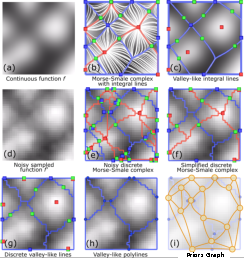
\includegraphics[width=0.6\columnwidth]{./figures/mscbackground.pdf}
 }
     \caption{ Morse-Smale complexes are defined for functions with continuous gradients {\bf(a-c)}. A smooth function {\bf(a)} can be partitioned based on the behavior of integral lines {\bf(b)}, with selected integral lines shown in white. This partition forms a cell complex, where integral lines within each cell share a common origin and destination. The 0-dimensional cells are  maxima (red), saddles (green), and minima (dark blue)), the 1-dimensional cells are formed by ascending (orange) and descending lines (light blue) from saddles (green), and 2-dimensional cells are bounded by 0- and 1-cells {\bf(b)}. Elements of this complex often form semantic features of interest in a scientific domain, such as valley-like lines {\bf(c)}. Real-world functions often come from noisy sources, and are available as samples on a grid {\bf(d)}. Discrete Morse-theory-based methods allow practical computation of Morse-Smale complexes {\bf(e)}, which encode both noise and discretization artifacts that may be simplified to recover the coarse-scale behavior of the function {\bf(f)}. The valley-like structures may be extracted from this complex {\bf(g)}, and converted to a set of priors between non-degree-2 vertices denoted the valley graph {\bf(h)}. The priors graph (yellow), {\bf(i)}, represents each prior as a vertex with edges between incident priors. }
     \label{mscbackground}

     \vspace{-.6cm}
     
 \end{figure}

\subsection{Topological Graph Hierarchy}
\label{ssec:topohier}

To model multiscale topological information, we compute the MSC at $P$ levels of persistence. In contrast to hierarchical graph-level representation learning methods that learn to pool each input graph~\cite{ying2018hierarchical}, this gives us several graph representations of the underlying data to use as input to a graph neural network. Computationally, a smaller persistence value produces a graph higher in the MSC hierarchy with higher granularity.  Thus, we obtain a hierarchy of graphs $G_1, \ldots, G_P$ where  $\forall p_i$ for $i \in [1, \ldots, P], G_{p_{i-1}} \subseteq G_{p_i}$: that is, $G_{p_{i-1}}$ is an induced subgraph defined on a subset of the vertices in $G_{p_i}$. %
%More formally, if we have persistence levels $p_i$ and $p_j$, such that $p_j < p_i$, then $\msc(p_i) \subset \msc(p_j)$ and $\iG \subset \jG$ for priors graphs $\iG$ and $\jG$. 
Node neighborhoods thus share this property: for each node $v_i \in \iV \cap \jV$, e.g. $\iNbr{v_i}$ for $v_i \in \iV$ and $\jNbr{v_i}$ for $v_i \in \jV$, we have that $\iNbr{v_i} \subseteq \jNbr{v_i}$. %Due to persistence filtrations resulting in a  sequential hierarchy of complexes and corresponding priors graphs,  
We give all graphs the full node set found at the lowest persistence level of the hierarchy, but nodes that would not otherwise exist in the graph at a higher persistence level are disconnected.%have isolated vertices without connections to any other vertex belonging to a graph of a higher persistence level.  

\iffalse
\begin{figure}[h!]
    \centering
    \resizebox{0.3\columnwidth}{!}{%
\includegraphics{figures/persistence_11_light_bg.png}
    }
    \caption{\red{Subgraph} used for hierarchical learning highlighted (in red) within \Blue{supergraph}.}
\label{fig:subgraph_pers11_neuron}
\end{figure}
\fi

